\chapter{Deep Neural Networks}
\label{chapter:dnn}

The history of artificial neural networks (ANN) dates back to 1943. In \cite{McCulloch1943} authors tried to mathematically describe the activity of biological neurons in the human brain. Using these principles they built the first artificial neuron and artificial neural network. In 1974 a PhD student, Paul Werbos, introduced in \cite{Werbos1974} the idea of backpropagation of errors by which ANN are able to learn other than linearly separable problems, and this idea was further expanded in \cite{Rumelhart1986}. Artificial neural networks that contain many hidden layers are also called deep neural networks (DNN) and the process of training this network is called deep learning \cite{LeCun2015}. Over the years deep learning and one of its variants - a convolutional neural network that was proposed in \cite{LeCun2015-2} - were found to be very effective and precise in domains that were found unreachable by the classical AI and ML algorithms \cite{LeCun2015}. This was caused by their ability to capture abstract and complex patterns that simpler models found impossible to catch. Such examples include analysis of image data \cite{Farabet2013, Alzubaidi2021} and recent advancements in natural language processing (NLP) \cite{Deng2018}.

\section{Structure}
The fundamental part of every artificial neural network is the neuron. Neuron is basically a function which has one or more inputs and one output. Inside this neuron, a mathematical computation is being done in order to transform input into output. Input can also be referred to as input vector or vector of input features. Each input feature has its weight by which it is multiplied. Next, a bias is added to the multiplied and summed features and weights. This calculation is still linear so in order for it to be able to capture more complex patterns, we need to apply a non-linear activation function to its output. The mathematical representation of artificial neuron can be seen in the equations \ref{eq:linear} and \ref{eq:activation} \cite{Goodfellow2016}.

\begin{align}
\label{eq:linear}
    z &= b + \sum_{i=1}^n (w_i x_i) \\
\label{eq:activation}
    a &= \varphi(z)
\end{align}

Where $z$ is the output produced by the linear unit, $b$ is the bias, $n$ is the number of input features, $x_i$ is the \textit{i}-th input feature, $w_i$ is the weight associated with the \textit{i}-th input feature, $a$ is the actual output, and $\varphi$ is the activation function.

Visual example of artificial neuron can be seen in figure \ref{fig:artificial-neuron}.

\begin{figure}[H]
\begin{centering}
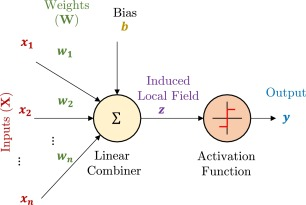
\includegraphics[width=8cm]{assets/images/neuron.jpg}
\par\end{centering}
\caption{Artificial neuron \cite{Santosh2022-1}}
\label{fig:artificial-neuron}
\end{figure}

\subsection{Activation Functions}
Activation functions are used to break linearity in neural networks - this enables them to capture more complex patterns, which are not linearly separable. Activation functions are used in combination with linear functions inside neurons. Different activation functions can be used, such as Sigmoid, Tanh, ReLU, ELU, GELU, and many more \cite{Dubey2022, Aby2025}.  The important part of an activation function is also its gradient, which is computed during backpropagation. 

\paragraph{Sigmoid}
Sigmoid is computed by the equation \ref{eq:sigmoid} and its derivative by the equation \ref{eq:sigmoid-derivative}. As we can see in figure \ref{fig:sigmoid} has a steep gradient around zero and it gradually flattens on both sides.

\begin{align}
\label{eq:sigmoid}
    \sigma(z) &= \frac{1}{1+e^{-z}} \\
\label{eq:sigmoid-derivative}
    \sigma^{'}(z) &= \sigma(z)(1-\sigma(z))
\end{align}

\begin{figure}[H]
\begin{centering}
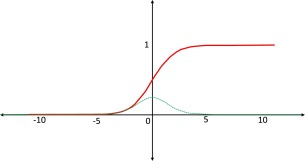
\includegraphics[width=8cm]{assets/images/sigmoid.jpg}
\par\end{centering}
\caption{Sigmoid activation function (red) and its derivative (green) \cite{Santosh2022-2}}
\label{fig:sigmoid}
\end{figure}

The output of the sigmoid is bound between zero and one, and its gradient can be used to push the output either closer to one or closer to zero \cite{Santosh2022-2}. It is often used for the output unit for the binary classification task, where the output is desired to be between zero and one \cite{Santosh2022-2, Goodfellow2016}.

\paragraph{Tanh} Next function is the \textit{tanh} activation function, given by the equation \ref{eq:tanh} and its respective derivative displayed on the equation \ref{eq:tanh-derivative}.

\begin{align}
\label{eq:tanh}
    \text{tanh}(z) &= \frac{e^z-e^{-z}}{e^z+e^{-z}} \\
\label{eq:tanh-derivative}
    \text{tanh}^{'}(z) &= 1-tanh^2(z)
\end{align}

Like the \textit{sigmoid} function, it compresses the input; however, unlike the \textit{sigmoid}, its output is constrained to the range of -1 to 1, as shown in figure \ref{fig:tanh}.

\begin{figure}[H]
\begin{centering}
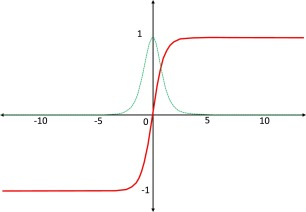
\includegraphics[width=8cm]{assets/images/tanh.jpg}
\par\end{centering}
\caption{Tanh activation function (red) and its derivative (green) \cite{Santosh2022-2}}
\label{fig:tanh}
\end{figure}

\paragraph{ReLU}
The problem with \textit{sigmmoid} and \textit{tanh} functions is the vanishing gradient and computational complexity. Vanishing gradient means that the gradient of a function is almost flat, hence close to zero, which leads to no or very little update in the network's learnable parameters (weights and biases) during the training \cite{Dubey2022, Aby2025}.

As a possible solution to these problems, a rectified linear unit, also known as ReLU, was introduced \cite{Nair2010}. ReLU is a simple function; its equation \ref{eq:relu} and derivative equation \ref{eq:relu-derivative} are straightforward.

\noindent
\begin{multicols}{2} % Two-column layout
    \begin{equation}
    \text{ReLU}(z) =
    \begin{cases} 
        z, & \text{if } z > 0, \\
        0, & \text{if } z \leq 0.
    \end{cases}
    \label{eq:relu}
    \end{equation}

    \begin{equation}
    \text{ReLU}'(z) =
    \begin{cases} 
        1, & \text{if } z > 0, \\
        0, & \text{if } z \leq 0.
    \end{cases}
    \label{eq:relu-derivative}
    \end{equation}
\end{multicols}

The ReLU function can be seen in figure \ref{fig:relu}. It basically returns its input if the input is positive otherwise, it returns zero. Since the derivative of \textit{x} is always one, the problem with vanishing gradient is solved. 

\begin{figure}[H]
\begin{centering}
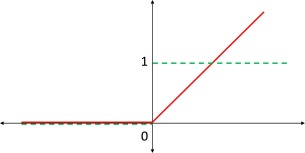
\includegraphics[width=8cm]{assets/images/relu.jpg}
\par\end{centering}
\caption{ReLU activation function (red) and its derivative (green) \cite{Santosh2022-2}}
\label{fig:relu}
\end{figure}

ReLU also introduces some potential drawbacks, i.e. the output for negative input is always zero. The problem called dying ReLU \cite{Dubey2022, Santosh2022-2, Aby2025} is when a negative input causes no updates in weights during training  and neurons in this state do not respond to error variations \cite{Santosh2022-2}. To fix this problem we can multiply the negative input value by a very small constant, which will allow the weights to be updated if it is needed. This modified ReLU is called Leaky ReLU \cite{Maas2013} and its formula and formula of its gradient are displayed in equations \ref{eq:leaky-relu} and \ref{eq:leaky-relu-derivative} respectively.

\noindent
\begin{multicols}{2} % Two-column layout
    \begin{equation}
    \text{LeakyReLU}(z) =
    \begin{cases} 
        z, & \text{if } z > 0, \\
        \alpha z, & \text{if } z \leq 0.
    \end{cases}
    \label{eq:leaky-relu}
    \end{equation}

    \begin{equation}
    \text{LeakyReLU}'(z) =
    \begin{cases} 
        1, & \text{if } z > 0, \\
        \alpha, & \text{if } z \leq 0.
    \end{cases}
    \label{eq:leaky-relu-derivative}
    \end{equation}
\end{multicols}

In addition to the Leaky ReLU, many other ReLU variants were introduced over the years, each bringing its own advantages, disadvantages, and challenges \cite{Dubey2022, Aby2025}.

Nowadays, the most commonly used activation function for hidden units is the ReLU activation function \cite{Dubey2022, Goodfellow2016, LeCun2015}.
% overview, traditional, new 

\subsection{Layers}

Similarly to biological neural networks, when artificial neurons are chained together, meaning the output from one neuron is passed to another neuron, they create an artificial neural network.

This network is organized in layers. Neurons in each layer are not connected together, but rather every neuron from layer \textit{L} is connected with every neuron from layer \textit{L+1}, except neurons in the first (input) layer. For better understanding, we will refer to the figure \ref{tab:artificial-nn} where we can see an example of a neural network.

\begin{figure}[H]
\begin{centering}
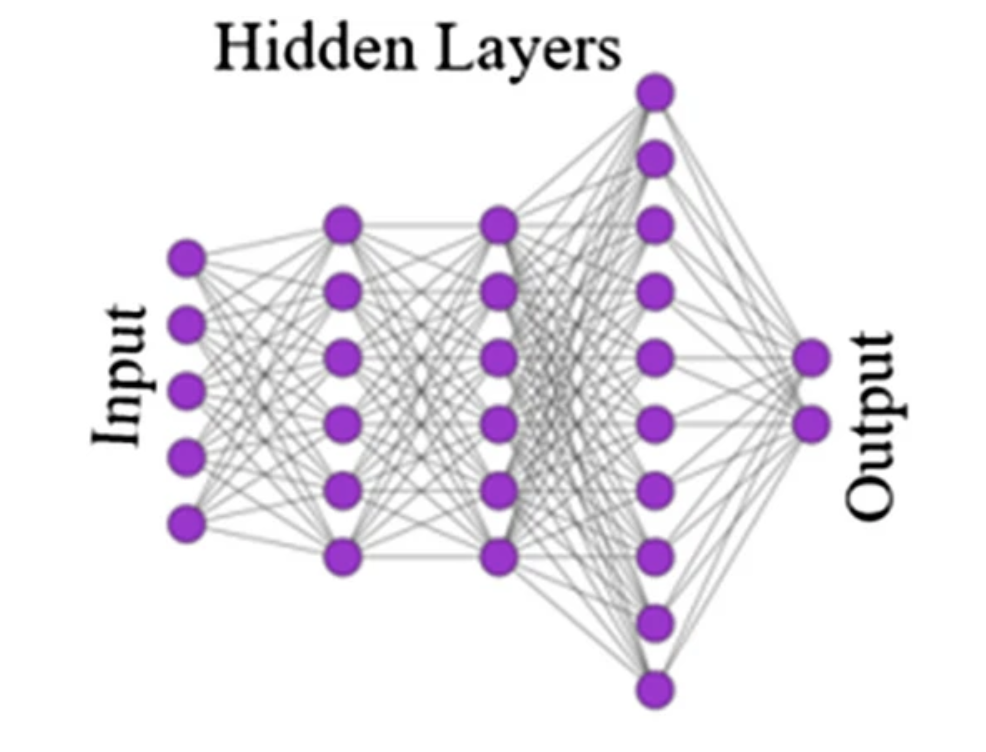
\includegraphics[width=8cm]{assets/images/neural_net.png}
\par\end{centering}
\caption{Example of deep artificial neural network \cite{TalaeiKhoei2023}}
\label{tab:artificial-nn}
\end{figure}

Neural network can be divided into three main parts:

\begin{itemize}
    \item Input layer
    \item Hidden layers
    \item Output layer
\end{itemize}

Input layer is the initial layer and the only layer that does not contain neurons which perform calculations but rather consists of \textit{N} input features $x_1, x_2, \dots, x_N$ also referred to as a vector $\vec{x}$ of input features displayed in equation \ref{eq:vector-input}.

\begin{equation}
\label{eq:vector-input}
\vec{x} = \begin{bmatrix}
x_1 \\
x_2 \\
\vdots \\
x_N
\end{bmatrix}
\end{equation}

The subsequent layers between the input layer and output layer are called hidden layers. The name comes from the fact that their outputs are not directly observable, nor are they provided by the external environment - they are internal to the network's architecture. Neurons inside these layers perform calculations on the input and produce output, which is then fed forward to the next layer \cite{LeCun2015}.

The final output layer produces an output of the network. Output and number of neurons depend on the task the network is being trained for. For regression tasks, one neuron is often suitable - it predicts a continuous variable \cite{Goodfellow2016}. During classification tasks, it can further depend on the nature of the classification. In binary classification, again a single neuron can suffice. It will display a probability of the input belonging to one of the classes - if the probability is high, it will assign that class to it, and if the probability is low, it will assign the other class to it \cite{Goodfellow2016}. In multi-class classification, the number of neurons is the same as the number of classes and each neuron predicts a probability of the input belonging to one specific class \cite{Goodfellow2016}.

\section{Loss Functions}
Loss function, sometimes also referred to as cost function, is a function that computes the difference between the result predicted by the model and the ground truth. This difference is called error. The error guides the model during training and is responsible for parameter updates. We are trying to find the local minimum of the cost function - a point where the error value is as low as possible, because this means that the model is making good predictions. Hence we are trying to find a global minimum of the cost function. Similarly to different activation functions, there is also a variety of cost functions.

\paragraph{Mean Squared Error}
Mean squared error (MSE) is computed as a sum of all differences between predicted output and real values (ground truth) raised to a power of two. The equation \ref{eq:mse} displays this computation, where $m$ is the number of input samples, $y$ is the ground truth, and $\hat{y}$ is the output predicted be the model. Despite being effective for regression problems, MSE is not that suitable for classification problems \cite{Santosh2022-2}.

\begin{align}
\label{eq:mse}
    E_\text{MSE} = \frac{1}{m}\sum_{i=1}^m(y_i-\hat{y}_i)^2
\end{align}

\paragraph{Cross-entropy Loss}
Much more efficient loss functions for classification problems are the entropy-based ones. For example, for binary classification, a logistic loss function, by which a binary cross-entropy error (BCE) is measured, is suitable \cite{Santosh2022-2}. It is given by the equation \ref{eq:logloss}, where $m$ is the number of input samples, $y$ is the ground truth, and $\hat{y}$ is the output predicted output.

\begin{align}
\label{eq:logloss}
    E_\text{BCE} = -\frac{1}{m}\sum_{i=1}^m(\hat{y}\log{y}+(1-\hat{y})(\log{(1-y)}))
\end{align}

This function can be modified to compute error for multiclass classification as well - this is also called categorical cross-entropy error (CCE). If we assume we have $C$ distinct classes we want to assign input into (and input can belong to exactly one class), then the equation \ref{eq:cce} computes the error. Here $m$ is the number of input samples, $C$ is a set of classes, $y_{i,c}$ is the ground truth for the \textit{i}-th sample and \textit{c}-th class, usually represented as a one-hot encoded vector where $y_{i,c}=1$ if the \textit{i}-th input belongs to the \textit{c}-th class, and $y_{i,c}=0$ and $\hat{y}_{i,c}$ is the predicted probability for the \textit{i}-th sample belonging to the \textit{c}-th class.

\begin{align}
\label{eq:cce}
    E_\text{CCE} = -\frac{1}{m}\sum_{i=1}^m\sum_{c=1}^C(y_{i,c}\log{\hat{y}_{i,c}})
\end{align}

\paragraph{Dice Loss}
The most popular choice for object segmentation task, and especially in the medical imaging domain, is the dice loss function \cite{Zhang2021}. It uses the Dice similarity coefficient (DSC) to compute the difference between predicted map $p$ and ground truth map $y$ for each class $j$ of $C$ classes. A slight problem exists with the DSC - it is not differentiable, therefore it cannot be used directly in training. To overcome this obstacle, neural networks use a probabilistic version of DSC to the discrete DSC in training \cite{Zhang2021}. Its computation is displayed in equation \ref{eq:dsc} where N depicts the number of pixels and $\epsilon$ is a small constant used to avoid division by zero. The computation of overall dice loss is displayed in equation \ref{eq:diceloss}, where $D_i$ is the DSC computed for the \textit{i}-th training sample.

\begin{align}
\label{eq:dsc}
\text{DSC}_i &= D_i = \frac{2 \sum_{n=1}^N \sum_{j=1}^C (y_{n,j} p_{n,j}) + \epsilon}{\sum_{n=1}^N\sum_{j=1}^C (y_{n,j} + p_{n,j}) + \epsilon} \\
\label{eq:diceloss}
E_\text{DiceLoss} &= \frac{1}{m}\sum_{i=1}^m (1-D_i)
\end{align}

\section{Training}
During the training phase, a neural network tries to minimize the cost function by adjusting its parameters - weights and biases. This process is often called learning, and we can say that the neural network learns to map input features onto the desired output. Prior to the training process we need to ensure that the data is in desired quality and quantity, otherwise the training will not be effective and the performance of the resulting model will be poor. Methods such as data preprocessing are typically used \cite{Goodfellow2016, LeCun2015}. 

The training itself consists of multiple steps:

\begin{enumerate}
    \item Parameter initialization
    \item Forward propagation
    \item Cost function computation
    \item Backpropagation and parameters updates
\end{enumerate}

\paragraph{Parameter initialization} During parameter initialization, we set the initial values of all learnable parameters of the network (parameters that can be updated during training). Different weight initialization strategies were developed, their overview can be seen in figure \ref{fig:init}.

\begin{figure}[H]
\begin{centering}
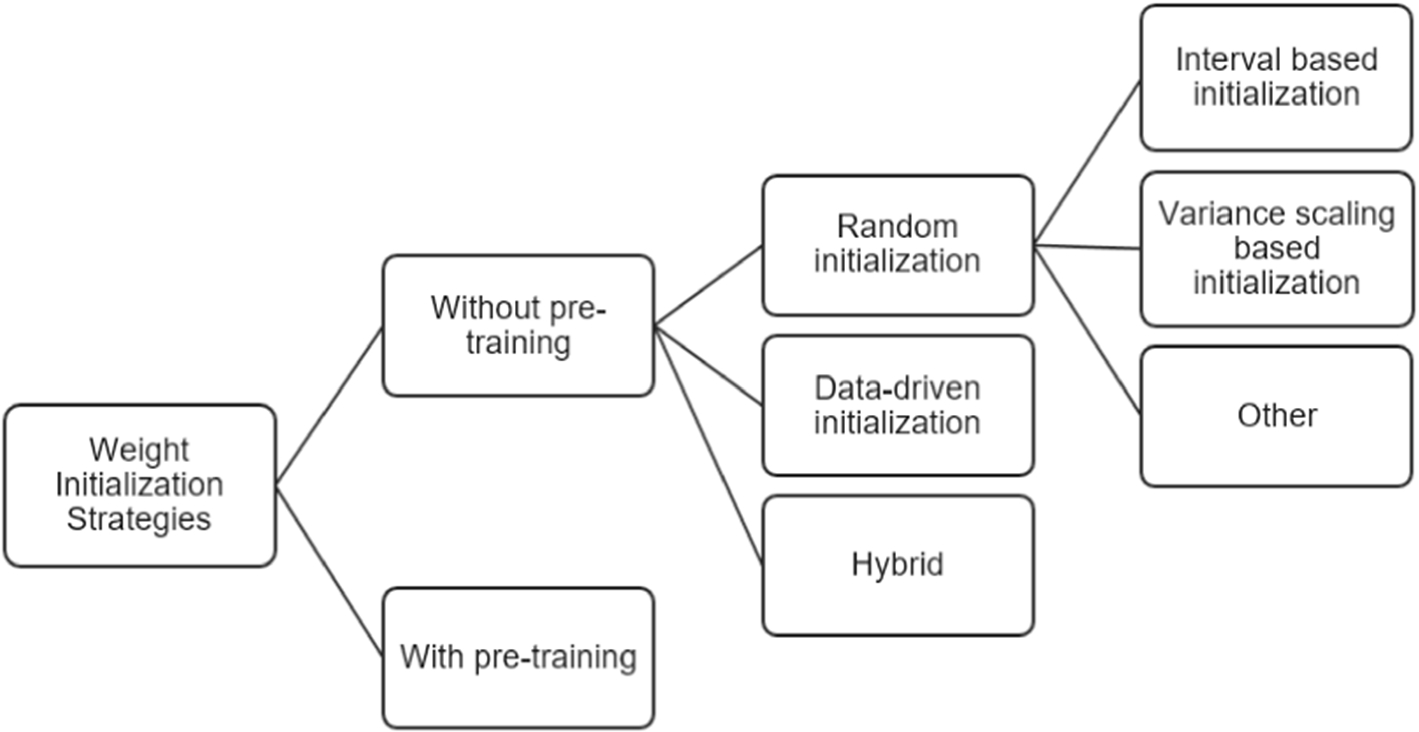
\includegraphics[width=8cm]{assets/images/init.png}
\par\end{centering}
\caption{Different weight initialization strategies \cite{Narkhede2021}}
\label{fig:init}
\end{figure}

Methods such as Xavier/Glorot or He initialization are also popular \cite{Abdullahi2023}.

\paragraph{Forward propagation}
During forward propagation the input sample data is fed forward through the layers of the network. For a hidden layer $L$ with $N$ neurons, and activation function $\varphi$:

\begin{itemize}
    \item The input is output from previous layer \textit{L-1} (the activations), denoted: $A_{L-1} \in \mathbb{R}^{m \!\times\! d}$, where $m$ is the number of input samples, and $d$ is the number of input features of each sample. Number $d$ is also equal to the number of neurons present in layer \textit{L-1}.
    \item Each neuron needs to have $d$ weights, one for each input feature. A weight matrix holding weights of all neurons in layer $L$ can then be denoted as: $W_L \in \mathbb{R}^{d \!\times\! N}$.
    \item Each neuron also holds a bias term, all biases in layer $L$ can be represented with vector $b_L \in \mathbb{R}^N$.
    \item Output matrix (the activations) returned by this layer can be denoted as: $A_L \in \mathbb{R}^{m \!\times\! N}$. This becomes input for the layer \textit{L+1}.
\end{itemize}

A computation performed by arbitrary hidden layer $L$ with $N$ neurons can that be calculated with equations \ref{eq:hidden-comp-z} - to compute $Z_L \in \mathbb{R}^{m \!\times\! N}$ pre-activation values, and \ref{eq:hidden-comp-a} - to compute output of layer $L$. Function $\varphi$ is applied element-wise on all elements of the input matrix.

\begin{align}
\label{eq:hidden-comp-z}
Z_L &= XW + b \\
\label{eq:hidden-comp-a}
A_L &= \varphi(Z)
\end{align}



The final output layer will then return the predicted output value for each sample. At the beginning of the training, the output values will be almost random, but as the training continues, the predicted values should converge towards the ground truth values - this is the desired behaviour \cite{Goodfellow2016, LeCun2015}.

\paragraph{Cost function computation}
After the sample (or samples) are fed forward through the network, we get either a matrix or vector of output values or a single output value. Next step is to compute the error of the network using one of the aforementioned cost functions, e.g. dice loss in case of image data. The error is than propagated backwards through the network and weights and biases are adjusted in a way that will minimize the cost function. This algorithm is called backpropagation \cite{Goodfellow2016}.

\paragraph{Backpropagation}
In order for network to learn, it should implement some kind of algorithm, that will adjust its learnable parameters (weights and biases) in a way, that the overall error will be lower next time the input samples are fed forward through the network. Backpropagation computes the gradients for each layer starting with the output layer, and by utilizing the chain rule of calculus, it propagates the error back through the network to the first hidden layer \cite{LeCun2015}.

After the gradients are computed, the parameters are updated accordingly by optimization algorithms such as stochastic gradient descent \cite{Santosh2022-2}. Formulas for updating weights and biases are shown in equation \ref{eq:w-update} and \ref{eq:b-update}, where $\alpha$ is a learning rate (which controls the speed of learning - if changes to the parameters are too great, the minimum can be missed, if changes are too small, the minimum will not be reached in a reasonable time) and $E$ is the cost function \cite{Goodfellow2016, LeCun2015}.

\begin{align}
\label{eq:w-update}
w &= w - \alpha \frac{\partial E}{\partial w} \\
\label{eq:b-update}
b &=  b - \alpha \frac{\partial E}{\partial b}
\end{align}

There is a strict rule for backpropagation to work - all functions used in the network must be differentiable at all points \cite{Rumelhart1986, Santosh2022-2}.

\subsection{Optimization and regularization}

\paragraph{Optimization}
There are many optimization techniques that are capable of further enhancing the model training and performance. Examples include:

\begin{itemize}
    \item using small batches of input samples and after each batch passes perform parameter updates,
    \item utilizing momentum \cite{Polyak1964} to have more control over the learning speed based on the previous gradients \cite{Santosh2022-2},
    \item using adaptive learning rates, where the learning rate $\alpha$ is usually great at the beginning and as the training progresses it is gradually reduced \cite{Santosh2022-2}. Updates to $\alpha$ can be done after some number of iterations by some preset factor or automatically by utilizing methods such as Adam (adaptive moments) \cite{Kingma2014} or RMSProp \cite{Zou2019}.
\end{itemize}

\paragraph{Regularization}
Another set of techniques that can improve model performance is regularization. Usually, a model's performance and prediction capabilities improve during training. Available data are often split into three subsets for training, validation, and testing. The model is, obviously, trained using the training subset. The validation subset is used to check model performance during training, and the test subset is used for the final evaluation of the model. It is important that both validation and test subsets contain samples the model has not yet seen during training - otherwise, the results would be biased. A good model should be robust and generalize well, not only learn patterns that are specific for training data. Sometimes, especially in more complex models, we can observe an effect when, at the beginning of the training, both training and validation performance (such as error value) improve, but later the validation performance plateaus or worsens - this effect is called overfitting \cite{Schaffer1993} and is displayed in figure \ref{fig:overfitting}. 

\begin{figure}[H]
\begin{centering}
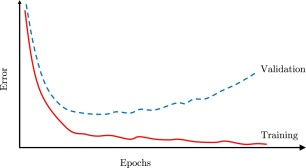
\includegraphics[width=8cm]{assets/images/overfitting.jpg}
\par\end{centering}
\caption{Error curve during training - overfitting happens \cite{Santosh2022-2}}
\label{fig:overfitting}
\end{figure}

This effect is not desired because it means that the model cannot generalize well on previously unseen samples - it is learning "by heart" from the training data. To overcome this problem, we can implement several regularization mechanisms, that will improve the model's robustness and ability to generalize. Examples include dropout \cite{Srivastava2014}, transfer learning \cite{Pan2009}, early stopping \cite{Sarle1996}, parameter norm penalties such as L1 regularization (lasso regression) and L2 regularization (ridge regression) \cite{Krogh1991}, and more \cite{Santosh2022-2}.



\section{Evaluation Metrics}
\label{chapter:dnn:eval}

When evaluating a model's performance, various different metrics exist that can be used. The evaluation metrics also depend on the task the model was trained for. During classification tasks, depending on the predicted and real values for each sample, we can differentiate four groups of results:

\begin{itemize}
    \item True Positives (TP) - a model assigns a sample to class $c$, when a sample belongs to class $c$,
    \item True Negatives (TN) - a model does not assign a sample to class $c$, when a sample does not belong to class $c$
    \item False Positives (TP) - a model does assign a sample to class $c$, when a sample does not belong to class $c$
    \item False Negatives (TN) - a model does not assign a sample to class $c$, when a sample does belong to class $c$
\end{itemize}

We will briefly describe some of the evaluation metrics in the following paragraphs. 

\paragraph{Accuracy, Precision, Recall, and F1-score} Calculation of these basic metrics is displayed in equations \ref{eq:accuracy}, \ref{eq:precision}, \ref{eq:recall}, and \ref{eq:f1}. They describe the relationships between the number of samples belonging to either the true positive (TP), true negative (TN), false positive (FP), or false negative (FN) groups.

\begin{align}
\label{eq:accuracy}
\text{Accuracy} &= \frac{TP + TN}{TP + TN + FP + FN} \\
\label{eq:precision}
\text{Precision} &= \frac{TP}{TP + FP} \\
\label{eq:recall}
\text{Recall} &= \frac{TP}{TP + FN} \\
\label{eq:f1}
\text{F1\ Score} &= 2 \!\times\! \frac{\text{Precision} \!\times\! \text{Recall}}{\text{Precision} + \text{Recall}}
\end{align}

\paragraph{Area Under the ROC Curve}
Receiver Operating Characteristics (ROC) Curve and area under it can be used as another evaluation metric for classification and is superior when compared to overall accuracy \cite{Bradley1997}. The ROC Curve is drawn in the ROC Space as a relationship between the True Positive Rate (TPR, Recall or Sensitivity) and False Positive Rate (FPR) at the different threshold levels \cite{Bradley1997, Nahm2022, Fawcett2006}; the calculation of TPR and FPR is shown in the equations \ref{eq:tpr} and \ref{eq:fpr}.

\begin{align}
\label{eq:tpr}
\text{FPR} &=\text{Specificity} = \text{Recall} = \frac{TP}{TP + FN} \\
\label{eq:fpr}
\text{FPR} &= 1-\text{Specificity} = \frac{FP}{FP + TN}
\end{align}

The ROC Space and example of ROC Curve is displayed in figure \ref{fig:roc}. Area under this curve (AUC - Area Under the ROC Curve) is then computed and interpreted:

\begin{itemize}
    \item if $\text{AUC} = 1$, this is the perfect model
    \item if $\text{AUC} = 0.5$, model capability is equal to random guess
    \item if $\text{AUC} < 0$, performance of the model is worse than the random guess
\end{itemize}

\begin{figure}[H]
\begin{centering}
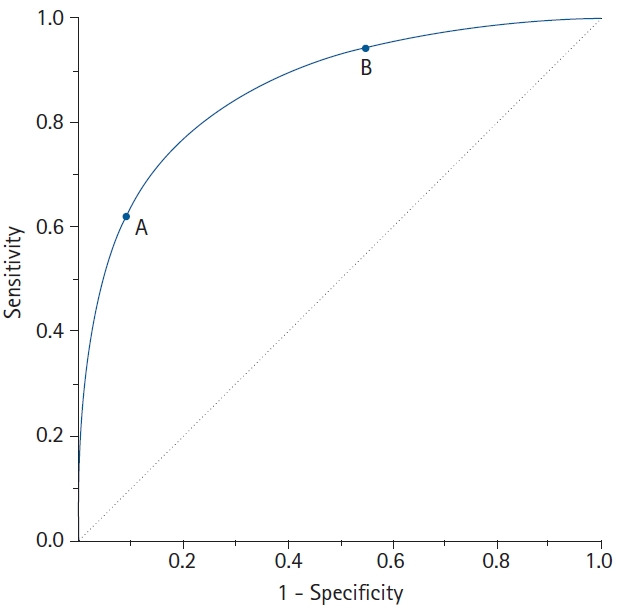
\includegraphics[width=8cm]{assets/images/roc-space.jpg}
\par\end{centering}
\caption{ROC Space with ROC Curve \cite{Nahm2022}}
\label{fig:roc}
\end{figure}

\paragraph{Intersection over Union} Intersection over Union (IoU), also known as the Jaccard Index, is a widely used evaluation metric in image segmentation and object detection \cite{Rezatofighi2019}. It is computed as the area of overlap between the predicted and ground truth regions divided by the area of their union. The closer the resulting value is to 1 the better the model predictions are \cite{Rezatofighi2019}. Its computation is shown in equation \ref{eq:iou}, where $y$ is the true area and $\hat{y}$ is the area predicted by the model.

\begin{align}
\label{eq:iou}
\text{IoU} &= \frac{y \cap \hat{y}}{y \cup \hat{y}}
\end{align}

\paragraph{Dice Coefficient} Similarly to the IoU, the Dice Coefficient is used for image segmentation and detection tasks \cite{Hu2023}, and the closer the resulting value is to 1 the better the model predictions are. Its computation is given by the equation \ref{eq:dice}, where $y$ is the true area and $\hat{y}$ is the area predicted by the model.

\begin{align}
\label{eq:dice}
\text{DiceCoefficient} &= \frac{2|y \cap \hat{y}|}{|y| + |\hat{y}|}
\end{align}

\section{Architectures}
\label{chapter:dnn-section:arch}
Neural network architectures like Convolutional Neural Networks \cite{LeCun2015-2} and U-Net \cite{Ronneberger2015} have proven to be effective in medical image analysis \cite{Santosh2022-2}. In recent years, also a concept of Vision Transformers \cite{Dosovitskiy2020, Hu2023} used in medical imaging shows promising results \cite{Shamshad2023, Hu2023, He2023}. In further sections, we describe each architecture and its contribution to the analysis of medical images and Digital Pathology.

\subsection{Convolutional Neural Networks}
In 1959, Hubel and Wiesel conducted experiments that inspired the advent of the Convolutional Neural Networks (CNN). In their experiments, they put a microelectrode into a cat's brain (into the part called the primary visual cortex), while it was under partial anesthesia. While showing various images to it, they measured the neurological activity of the cortex \cite{Hubel1959}. According to the results, a hierarchical pattern can be observed in the activity of the visual cortex, where the neurons close to the retina captured the simplest patterns (like different illuminations and lines under various angles) and the farther layers captured more complex patterns (like geometric shapes and other complex visual patterns) \cite{Hubel1959}. 

CNN took advantage of these findings and rebuilt the classical neural network layers to be able to capture more complex features with increasing depth. They utilize so-called convolution layers along with the ReLU activation function to learn to extract relevant features from the image. The deeper the convolution layer, the more complicated features it can learn \cite{Santosh2022-2}. 

Similarly to the Hubel and Wiesel cat's visual cortex, the first layers can learn to identify basic shapes like lines and simple geometric shapes, and the deeper layers can learn to identify more complex ones. Such an example of CNN is shown in figure \ref{fig:cnn}.

\begin{figure}[H]
\begin{centering}
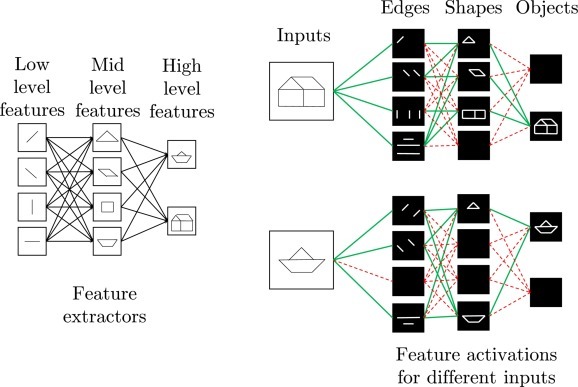
\includegraphics[width=10cm]{assets/images/cnn.jpg}
\par\end{centering}
\caption{Example of CNN learning strategy \cite{Santosh2022-2}}
\label{fig:cnn}
\end{figure}

A convolution layer applies a series of operations on its input and produces an output map. The most important part is applying a kernel, which is a tensor of fixed width and height, over the input image or output map from the previous convolution layer. This fundamental operation serves as a feature-extracting technique. The kernel slides over its input across its height and width and at each step, it performs element-wise multiplication of the pixel values it currently overlaps at each layer of depth and then sums them together to produce a single value. So, for example, if the input is of size $100\!\times\!100\!\times\!3$ (standard RGB image with 3 channels for red, green, and blue color), then the kernel is applied to all three channels simultaneously. After the kernel is applied to the whole image, the resulting output map will be of size $100\!\times\!100\!\times\!1$ (assuming that other hyperparameters of convolution are configured in such a manner that the original width and height remain unchanged for the output map - we will cover them later in this chapter), because the kernel will collapse its depth. 

The kernel filters can be handcrafted to multiply and intensify certain properties of the image. Examples include the Prewitt, Gabor, Sobel, Laplacian, and Roberts filters for edge and gradient detection. In standard image processing, the weights inside of the kernel are preset. However, in the CNNs these weights are learned during training, so the network determines what features of the image the output maps will be focused on and hence the network can be more effective \cite{Santosh2022-2, He2023}. In the AlexNet \cite{Krizhevsky2012}, the first deep CNN which outlined the original structure, a ReLU activation function was applied to the value obtained from the convolution operation to break the linearity of the operation. Since then, using an activation function after the convolution operation has become a standard practice \cite{Santosh2022-2, He2023}, and the name of the output produced by the convolution + ReLU is also called an activation map.

According to the \cite{Santosh2022-2}, convolution operation can be expressed as a function with hyperparameters: $\varphi_{\text{conv}}(C_{\text{in}}, C_{\text{out}}, K, S, P, D)$. The definition of these hyperparameters is:

\begin{itemize}
    \item $C_{\text{in}}$ is the number of channels of the input map - its depth.
    \item $C_{\text{out}}$ is the number of channels of the output produced by the layer - it is also the number of filters that will be applied to the input map since one filter produces an activation map with one channel.
    \item $K$ is a tuple that defines the size of the kernel - its width ($k_w$) and height ($k_h$)
    \item $S$ is also a tuple, which defines the stride - the number of pixels the kernel will slide along with, both in terms of width and height.
    \item $P$ can also be a tuple and it defines the number of added dummy pixels to artificially increase the input map size in order for the output map to keep the same size as the input map (otherwise the output map would be smaller since the kernels cannot slide outside of the boundary of the input map).
    \item $D$ (a tuple as well) is the dilation and it serves the purpose of increasing the field of view of the kernel (the area of the image it can cover) without adding more weights to it. Dilation defines the gap that is added both horizontally and vertically between the weights of the kernel.
\end{itemize}

We can see an example of the convolution in the figure \ref{fig:convolution}.

\begin{figure}[H]
\begin{centering}
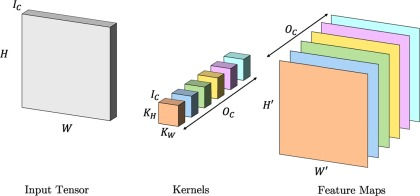
\includegraphics[width=8cm]{assets/images/conv.jpg}
\par\end{centering}
\caption{Example of the convolution operation \cite{Santosh2022-2}}
\label{fig:convolution}
\end{figure}

The field of view of a single kernel is small, as typically kernels of size $3\!\times\!3$, $5\!\times\!5$, or $7\!\times\!7$ are used \cite{Santosh2022-2}. In order to address this issue and to be able to build up and capture more complex features in the subsequent layers, the pooling layer is often added. The pooling layer effectively downsamples the feature maps, commonly by a factor of two. This allows the next convolution layers to learn more abstract features that were further apart in the previous feature map. In order to compensate the information lost during the downsampling, usually a number of independent kernels is increased for the next convolutions after each pooling layer. During pooling, a small array slides over the input map and always selects only a single value from the area it covers, hence decreasing the size of the map. Two pooling methods are common:

\begin{enumerate}
    \item Max pooling selects the maximal value from the area it covers, and
    \item Average pooling computes the mean from the values it covers.
\end{enumerate}

Example of pooling, both max and average, can be seen in the figure \ref{fig:pooling}.

\begin{figure}[H]
\begin{centering}
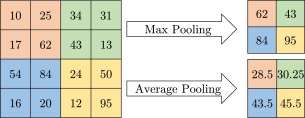
\includegraphics[width=8cm]{assets/images/pooling.jpg}
\par\end{centering}
\caption{Example of max and average pooling operations \cite{Santosh2022-2}}
\label{fig:pooling}
\end{figure}

CNNs are usually organized as repeating layers of convolutions, followed by the ReLU activation function and then the pooling layer. The output can be then fed into another convolution and a deep CNN can be built using this approach. There is a rule of thumb \cite{Santosh2022-3}, where we start with a small number of independent filters with a small field of view, and then we downsample the image by the factor of two (to increase the field of view) and double the subsequent number of independent filters as can be seen in figure \ref{fig:cnn-layers}.

\begin{figure}[H]
\begin{centering}
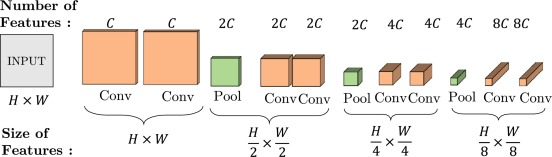
\includegraphics[width=12cm]{assets/images/cnn-layers.jpg}
\par\end{centering}
\caption{Scale space pyramid of a CNN \cite{Santosh2022-3}}
\label{fig:cnn-layers}
\end{figure}

In CNNs with very large depth, a concept of a skip connection, firstly introduced in the \cite{He2016}, can be used. A skip connection allows the input of a layer to bypass the convolutions and then be added to their result, as shown in figure \ref{fig:skip-conn}. Also, if we can represent a series of convolutions with a function $\varphi(x)$, then the output with skip connection included would be given by $y=\varphi(x) + x$. This residual learning architecture can mitigate the problem of vanishing gradient in very deep CNNs \cite{Santosh2022-2}.

\begin{figure}[H]
\begin{centering}
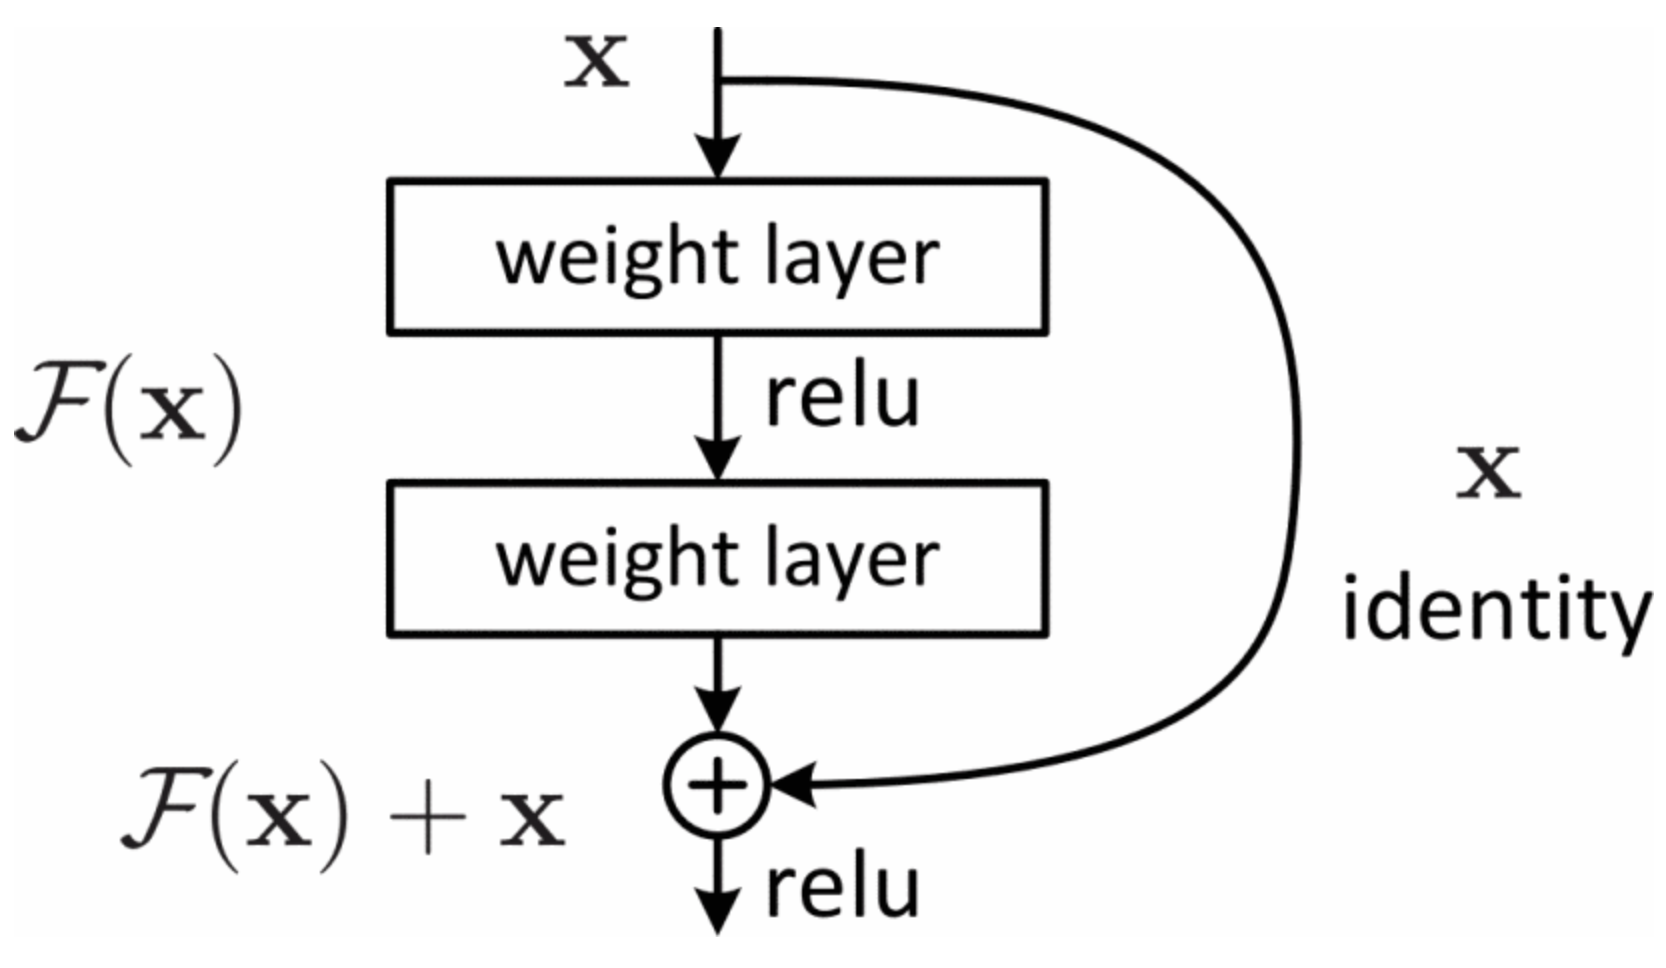
\includegraphics[width=8cm]{assets/images/skip-conn.png}
\par\end{centering}
\caption{A building block of residual network \cite{He2016}}
\label{fig:skip-conn}
\end{figure}

Other strategies that can improve the performance of CNNs include batch-normalization layers \cite{Ioffe2015}(which are inserted after the convolution layers) and the utilization of parallel branches \cite{Szegedy2015} (which use different kernel sizes to compute multi-scale feature maps by concatenating their output maps).

After the series of convolutions and downsampling, the final compressed feature representation of the image needs to be flattened (converted into a vector) so it can serve as an input for the fully connected layer(s), which will then make the appropriate decision based on the task the model should do. Two methods exist \cite{Santosh2022-2}, how we can convert the image descriptor into a vector:

\begin{enumerate}
    \item Reshape the activation maps to form a one-dimensional tensor \cite{Krizhevsky2012, LeCun2015-2}.
    \item Use average pooling on the entire activation map which will collapse the entire information into a single value and then concatenate these values to form a vector. For $N$ activation maps we will get a vector with $N$ elements \cite{He2016, Szegedy2015}.
\end{enumerate}

We can see their visual representation in figure \ref{fig:flatenning}.

\begin{figure}[H]
\begin{centering}
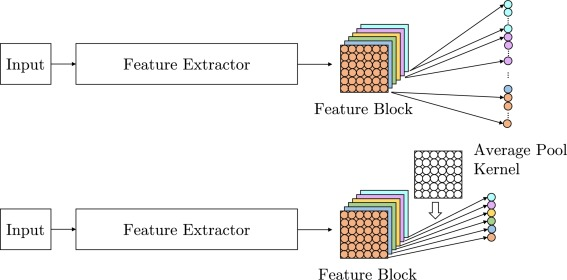
\includegraphics[width=12cm]{assets/images/flattening.jpg}
\par\end{centering}
\caption{Different flattening strategies \cite{Santosh2022-2}}
\label{fig:flatenning}
\end{figure}

An example of a CNN with all layers is in figure \ref{fig:full-cnn}. The input image features are extracted by the convolution layer with four independent $5\!\times\!5$ kernel filters, followed by the ReLU activation function and max pooling layer. Then the extracted image descriptor is flattened into a vector and fed into fully connected layers which serve as the classification output head.

\begin{figure}[H]
\begin{centering}
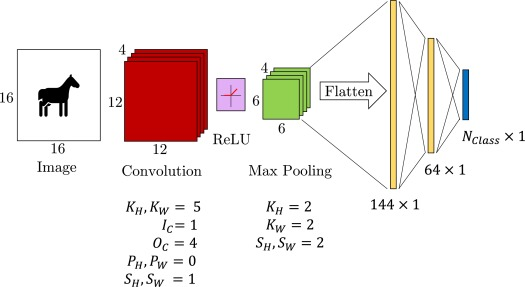
\includegraphics[width=10cm]{assets/images/cnn-full.jpg}
\par\end{centering}
\caption{Example of CNN architecture \cite{Santosh2022-2}}
\label{fig:full-cnn}
\end{figure}

There are many CNN architectures that introduced new concepts in the field of computer vision and image analysis when they were presented. Considering today's knowledge and advancements, some of them might look trivial, but their contribution should not be overlooked. In the classification task, we can mention:

\begin{enumerate}
    \item LeNet5 \cite{LeCun2015-2}: uses a series of convolution and pooling operations to extract the image features and fully connected layers to classify the input. It was introduced as a model that should recognize handwritten digits.
    \item AlexNet \cite{Krizhevsky2012}: built on top of the LeNet, utilized a deeper architecture along with ReLU activation functions, and had immense success at the ImageNet Large-Scale Visual Recognition Competition. This success brought huge attention to the  CNNs and their potential in image analysis-related tasks.
    \item VGGNet \cite{Simonyan2014}: introduced a strategy of expandable convolutional blocks, where in each block a varying number of convolutions can be used. Each block is then followed by the max pooling layer. This allowed for tailoring the network to reflect the complexity of the problem it was assigned to solve.
    \item GoogleLeNet \cite{Szegedy2015}: used kernels of varying sizes to extract features from the input maps and then concatenated their output maps to create a depth-wise combined feature. It also used the full-scale average pooling in the final feature extracting layer to create a one-dimensional tensor. Furthermore, it utilized auxiliary classifiers in the intermediate layers to boost the gradient flow. The later version, called Inception Net, introduced more concepts, like kernel factorization and batch normalization \cite{Szegedy2016-2}.
    \item ResNet \cite{He2016}: introduced a strategy of skip connections to solve the problem of vanishing gradient in very deep CNNs. 
\end{enumerate}

In the detection task, two main architectures were created, namely the Region-based CNN \cite{Girshick2014} (further upgraded to the Faster R-CNN and Mask R-CNN \cite{Ren2017}) and the You Only Look Once (YOLO) \cite{He2017}. 

Both R-CNN and YOLO are able to localize the object in an image with a bounding box label. However, sometimes we want to obtain a more precise location of the object, and this is where segmentation comes into play.

\subsection{U-Net and Its Variants}
In order to perfectly localize an object in an image, we would like to construct a pixel-level mask that would mark the pixels where the object is present. We can use classification for this - each pixel can either be classified as the one that does or does not display a part of the object. Segmentation algorithms have a deep impact and huge potential for medical imaging and digital pathology, where they can be used to mark different tissue types, organs, cells, and tumor regions \cite{Santosh2022-3}.

The limitation of full CNN architectures is the inability to preserve the spatial information after the initial feature-extracting layers \cite{Santosh2022-3}. This issue is addressed in a new type of architecture, the encoder-decoder architecture. This architectural type, also known as the autoencoders or auto-associative networks, was first introduced in the \cite{Kramer1992}. Its visual representation is shown in figure \ref{fig:autoencoder}.

\begin{figure}[H]
\begin{centering}
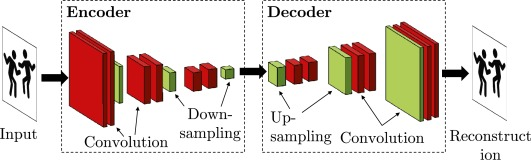
\includegraphics[width=12cm]{assets/images/encoder-decoder.jpg}
\par\end{centering}
\caption{Example of the autoencoder architecture \cite{Santosh2022-2}}
\label{fig:autoencoder}
\end{figure}

It consists of two main parts:

\begin{enumerate}
    \item The encoder part, which is responsible for encoding the input image and extracting the most descriptive features, compressing them and reducing the redundancy, and
    \item The decoder part, is responsible for reconstructing the original input image from the compressed image descriptor.
\end{enumerate}

The loss function computes the difference between the original input image and the image constructed by the decoder. If the decoder is able to create an image that looks very similar to the original, it means that the hidden representation of the image extracted by the encoder is credible enough. Then the decoder part can be removed and instead, a classification, segmentation, or localization module can be attached and exploit the features learned by the encoder \cite{Santosh2022-2}.

In segmentation tasks, a simple change is added to the decoder part. Instead of generating the original image, it is trained to create the segmentation mask, where each pixel has a probability of belonging to a certain class. This computed probability distribution mask is used along with the original mask in the loss function to compute their difference and guide the training.

When the activation maps are downscaled in the encoder using operations such as max pooling, where only a single value is picked, we need a correct mechanism to reconstruct the original spatial position of that value during the upscaling of the maps. This can be achieved by remembering and forwarding the indices of the chosen value, as it was first introduced in the SegNet architecture \cite{Badrinarayanan2017}.

One of the most widely adopted and impacting architectures is the U-Net model \cite{Ronneberger2015}. U-Net was designed as the model for medical image segmentation tasks and achieved great success in doing so \cite{Santosh2022-3, Siddique2021}. Its architecture can be seen in figure \ref{fig:unet}.

\begin{figure}[H]
\begin{centering}
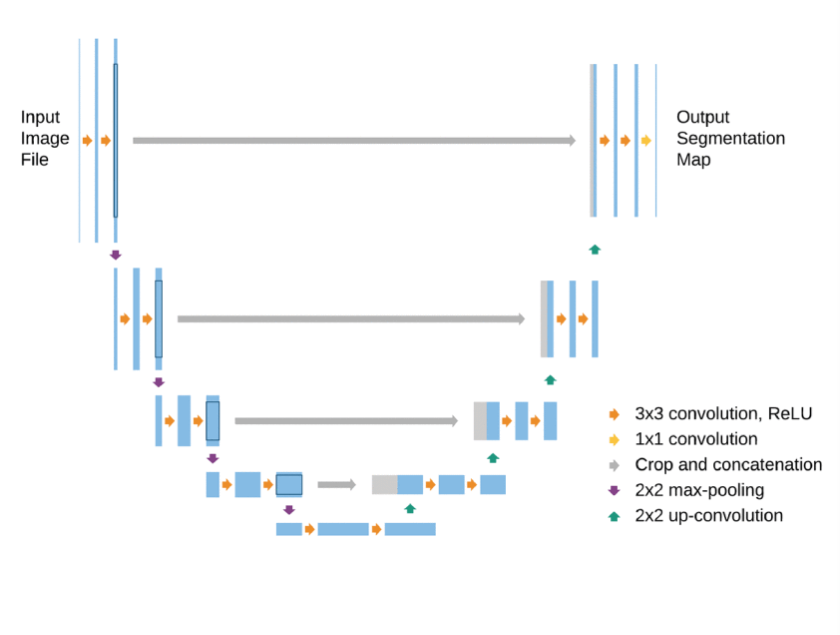
\includegraphics[width=12cm]{assets/images/unet.png}
\par\end{centering}
\caption{U-Net architecture \cite{Siddique2021}}
\label{fig:unet}
\end{figure}

Similarly to autoencoders, it has two main parts, the encoder and decoder. The encoder works as a classical CNN feature extractor, with convolutions, ReLU activation functions, and max pooling. In each layer there are two convolutions (kernel size is $3\!\times\!3$), followed by the ReLU, and the resulting activation maps are downsampled by the factor of two using the max pooling layer (with $2\!\times\!2$ matrix). Before the downsampling happens, the copy of the activation maps is sent to the decoder (skip connections). Every next block doubles the number of channels. This is repeated four times until we reach the bottleneck, where we again perform the convolutions with ReLU, but omit the downscaling. At this point, the features of the input image are in their most compressed form. Output from the bottleneck is then sent to the decoder part. Next, the decoder part uses up-convolutions (kernel size is $2\!\times\!2$), to expand the feature maps (double their size) and halve the number of channels. Particularly these up-convolutions are distinctive when comparing U-Net to other architectures \cite{Siddique2021}. The activation map is upscaled by up-convolution, and then the activation maps, previously sent from the encoder, are concatenated with it. The concatenation is a required step since the border pixels are lost in every convolution (the convolutions do not use padding), and also to reintroduce some information that might be lost during the downsampling. Then again two $3\!\times\!3$ convolutions with ReLU are applied. This is also repeated four times, to reflect the encoder blocks. This approach can be visually drawn into a U-shape-like architecture, from which the U-Net derived its name. Finally, after the last decoder block, the $1\!\times\!1$ convolution is used to get the desired number of channels.

Since the original U-Net, many different variants of it have been introduced \cite{Siddique2021}. To list a few examples:

\begin{itemize}
    \item 3D U-Net \cite{Çiçek2016}: works as a classical U-Net but was modified in a way that it can segment 3-dimensional data. Every 2D operation (2D convolution, 2D pooling, 2D up-convolution) was replaced by their corresponding  3D equivalents. It can be useful in medical images that utilize 3D space like MRI and CT.
    \item Attention U-Net \cite{Oktay2018}: utilizes the attention gate to draw the attention of the network to the important parts of the image. These attention gates are inserted in a place where the concatenation of encoder feature maps and decoder feature maps should occur, as can be seen in figure \ref{fig:att-unet}. Before this concatenation happens, both sets of feature maps are run through the attention gate where a series of operations is performed. These operations are visualized in figure \ref{fig:att-gate}. Firstly both sets are run through a $1\!\times\!1\!\times\!1$ convolution to align their dimensions and then are added together. Then they pass through the ReLU activation function, $1\!\times\!1\!\times\!1$ convolution layer to reduce their depth to 1, the sigmoid activation function to squeeze the values between 0 and 1, and an optional resampler to correctly align the spatial dimensions. This results in an attention map containing values between 0 and 1 and with a depth of 1. This attention map is then broadcasted and multiplied by the feature maps from the encoder - this produces the final output of the attention gate, which is then concatenated with the feature maps upsampled by the decoder.

    \begin{figure}[H]
    \begin{centering}
    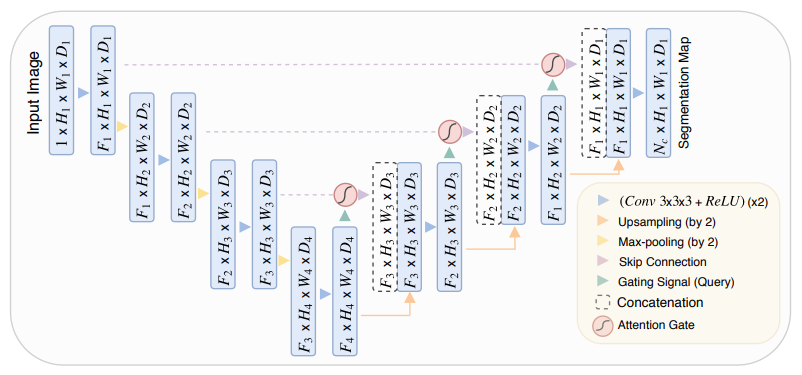
\includegraphics[width=12cm]{assets/images/att-unet.png}
    \par\end{centering}
    \caption{U-Net architecture with added attention gates \cite{Oktay2018}}
    \label{fig:att-unet}
    \end{figure}

    \begin{figure}[H]
    \begin{centering}
    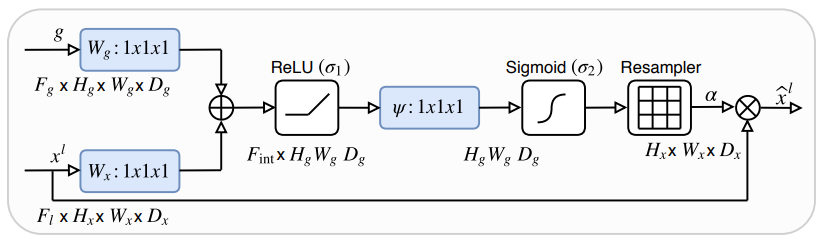
\includegraphics[width=12cm]{assets/images/att-gate.png}
    \par\end{centering}
    \caption{Additive attention gates \cite{Oktay2018}}
    \label{fig:att-gate}
    \end{figure}

    \item Residual U-Net is inspired by the \cite{He2016} and uses the skip connections within each block to help the gradient flow and address the problem of vanishing gradient.
\end{itemize}

Many more U-Net variants exist that we do not explain further in this work, for example, the Inception U-Net, Recurrent U-Net, Dense U-Net, Adversarial U-Net, Ensemble U-Net, and $\text{U-Net}^{++}$, each showing potential in various medical imaging domains, from CT and MRI scans to radiology, cytology, and histology \cite{Siddique2021}.

\subsection{Vision Transformers}
CNNs were for a long time considered the dominating architectural pattern in deep learning tasks related to visual data, similar to the RNNs being dominant in sequential data processing such as natural language processing (NLP) \cite{Vaswani2017}. When the Transformer architecture was proposed in \cite{Vaswani2017}, things began to change. Nowadays, transformer-based architecture is prevalent in the NLP field \cite{Shamshad2023} and with the introduction of Vision Transformer in \cite{Dosovitskiy2020} it seems, that transformers can be applied in computer vision as well and potentially compete with CNNs \cite{Hu2023}.

Vision Transformers (ViTs) build on the success of Transformers in NLP tasks \cite{Dosovitskiy2020, Shamshad2023}. Transformers utilize the attention mechanism that is able to capture a global context of the input data and is not limited by the distance of the pixels as was the case of CNNs \cite{Shamshad2023}. ViTs took advantage of the standard transformer encoder part which can be seen in figure \ref{fig:vit}. The encoder connects together multiple attention blocks to make use of the global image context.

\begin{figure}[H]
    \begin{centering}
    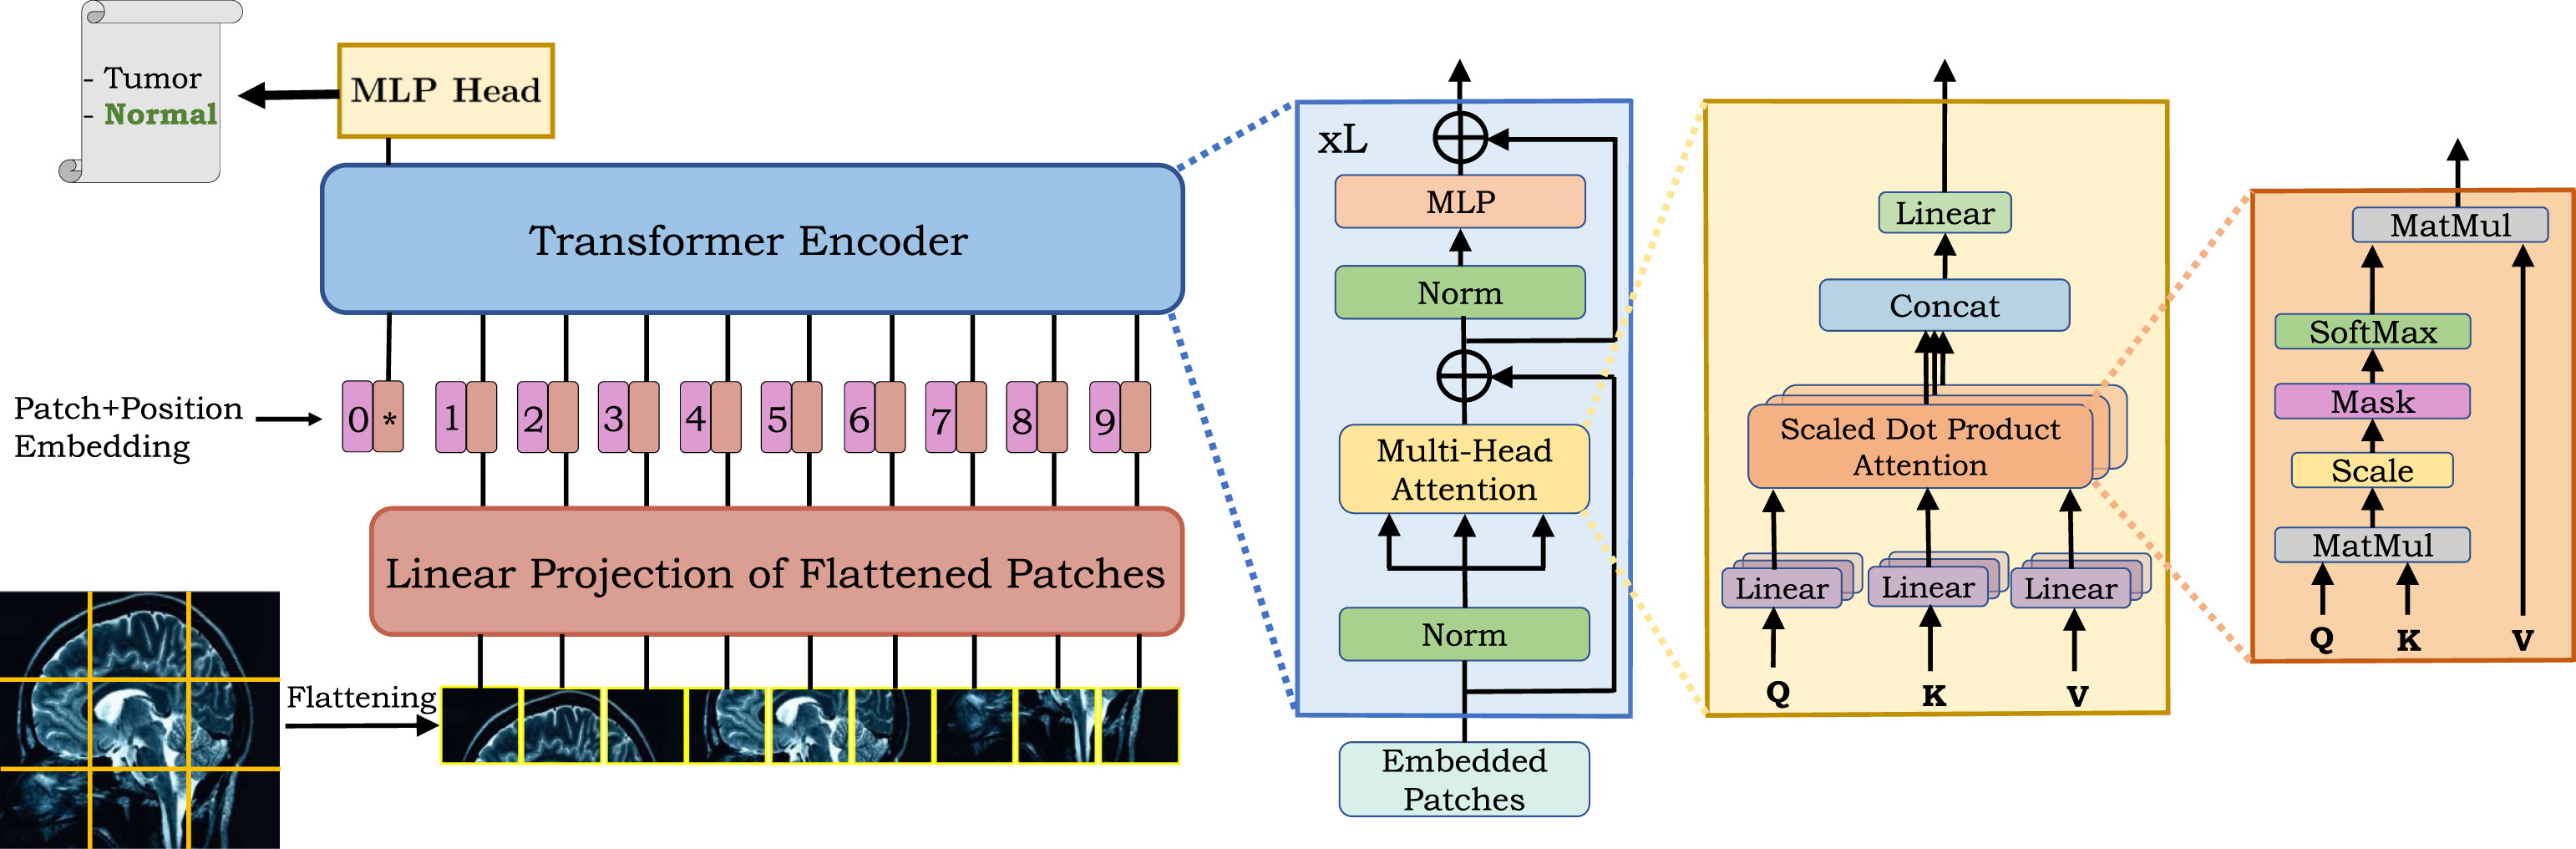
\includegraphics[width=14cm]{assets/images/vit.jpg}
    \par\end{centering}
    \caption{Vision transformer architecture for classification \cite{Shamshad2023}}
    \label{fig:vit}
\end{figure}

Below we briefly mention the ViT algorithm as described in \cite{Shamshad2023}:

\begin{enumerate}
    \item The input image is split into patches with fixed sizes, for example, authors in \cite{Dosovitskiy2020} used patch size of $16\!\times\!16$ pixels
    \item Image patches are converted by flattening into the vector space
    \item To reduce the dimensions of the resulting embeddings, vectorized patches are run through a trainable linear layer
    \item Since transformers are not aware of the spatial information, positional information is added to each vectorized embedding
    \item This sequence is then fed into the encoder
    \item Since ViTs require a huge amount of data to perform well, it is a great idea to pre-train the ViT on a large dataset and then fine-tune it to the specific task.
    \item In classification tasks, an extra embedding is added which will be learned during training - the class embedding.
\end{enumerate}

The self-attention mechanism and multi-head self-attention are the key components of ViTs success. The self-attention mechanism allows the model to figure out the importance of a patch embedding with respect to all the other patch embeddings of the image. The multi-head self-attention is composed of multiple self-attention units (also called heads) where each head is independent of the other heads. In the end, their outputs are stacked onto one another and passed through another linear layer. Skip connections facilitate better gradient flow and are added after the multi-head attention unit and before the final output. The produced output can serve as input to another attention block, hence a deep network can be constructed. This allows the model to capture complex relationships and dependencies across the input embeddings \cite{Shamshad2023}.

Vision Transformers have achieved great success along with CNNs in many applications of the medical imaging domain in tasks such as medical image classification, segmentation, restoration, synthesis, medical object detection, and more \cite{Shamshad2023}.

%\section{Active Learning}
%Deep learning models performing supervised learning, although achieving great performance, require a substantial amount of labeled data. In the medical imaging domain it is even harder to collect a dataset with high-quality annotations \cite{Nath2021}. 

%The concept of active learning can serve as a potential solution to this problem \cite{Nath2021, Wang2023}. Pool-based active learning is a standard active learning strategy \cite{Wang2023}. In this methodology, a model is trained with a smaller set of annotated data and then we let it predict the labels of samples in the unlabeled dataset (we call this also a pool of unlabeled data). Then those samples are selected, which have the greatest informative value and potential to improve the model in the next iteration of training. Different selection strategies exist, for example, we can select those samples that the model was least certain about (uncertainty sampling), or we let a set of models do the labeling and select those samples, in which there was the greatest disagreement among the models (query-by-committee) \cite{Wang2023}. These samples are then sent to the oracle (e.g. medical professional) for labeling and are added back into the annotated dataset and after enough samples are annotated by the oracle, the model is retrained \cite{Wang2023}. A visual example of this process can be seen in figure \ref{fig:active-learning}.

%\begin{figure}[H]
%    \begin{centering}
%    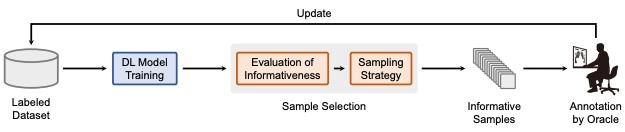
\includegraphics[width=14cm]{assets/images/active-learning.png}
%    \par\end{centering}
%    \caption{Active learning in medicine \cite{Wang2023}}
%    \label{fig:active-learning}
%\end{figure}

